\titledquestion{Array Representation of Linked-List}

Recall that we stored a linked-list in an array to avoid memory allocation problems in the lecture. In this question, we use two arrays: \ttt{next} and \ttt{value} to implement a singly-linked-list.

The elements at each index in \ttt{next} and \ttt{value} are together to represent a node in the linked-list, where \ttt{next} represents the array index where the next node is located (\(-1\) for already reaching the tail), and \ttt{value} represents the data stored in the node.

\tikzstyle{listnode} = [circle, draw = black]

\begin{parts}
	\part[5] \textbf{Store a Linked-List in an Array}\par
	Fill in the table below to finish the array representation of the linked-list shown below. Fill in \(-1\) to represent the end of the linked-list.
	\begin{center}
		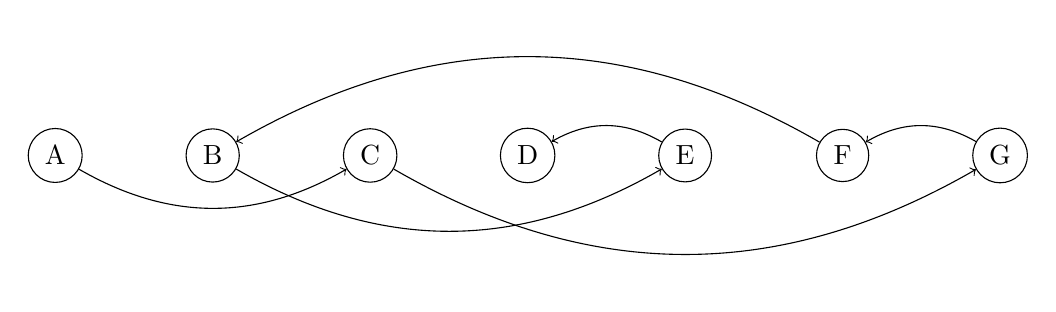
\begin{tikzpicture}[node distance = 2cm]z
			\node[listnode] (A) {A};
			\node[listnode, right of = A] (B) {B};
			\node[listnode, right of = B] (C) {C};
			\node[listnode, right of = C] (D) {D};
			\node[listnode, right of = D] (E) {E};
			\node[listnode, right of = E] (F) {F};
			\node[listnode, right of = F] (G) {G};
			\path[->]
			(A) edge[bend right] node {} (C)
			(C) edge[bend right] node {} (G)
			(G) edge[bend right] node {} (F)
			(F) edge[bend right] node {} (B)
			(B) edge[bend right] node {} (E)
			(E) edge[bend right] node {} (D);
		\end{tikzpicture}\par
		\begin{tabular}{|c|c|c|c|c|c|c|c|}
			\hline
			index       & 0 & 1 & 2 & 3  & 4 & 5 & 6 \\
			\hline
			\ttt{value} & A & B & C & D  & E & F & G \\
			\hline
			%%%%%%%%%%%%%%%%%%%%%%%%%%%%%%%%%%%%%%%%%%%%%%%%
			% YOUR ANSWER HERE.
			\ttt{next}  & 2 & 4 & 6 & -1 & 3 & 1 & 5 \\
			%%%%%%%%%%%%%%%%%%%%%%%%%%%%%%%%%%%%%%%%%%%%%%%%
			\hline
		\end{tabular}
	\end{center}

	\part[5] \textbf{From Array to Linked-List}\par
	Here are the arrays \ttt{next} and \ttt{value}. Please draw the linked-list below represented by these two arrays.
	\begin{center}
		\vspace{1.5cm} % space above (You may remove this.)
		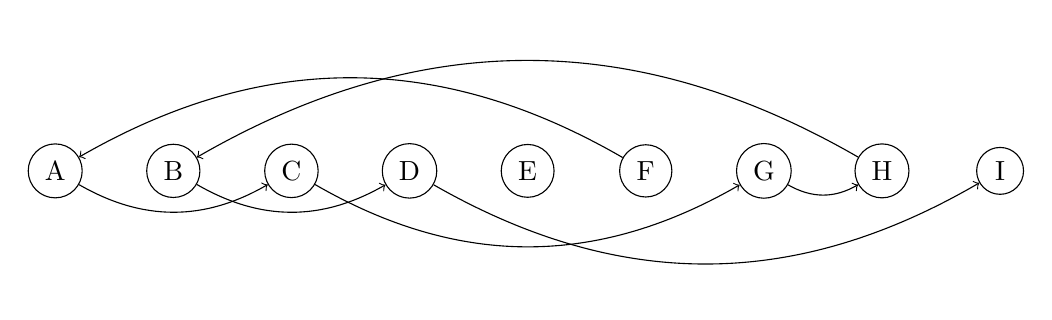
\begin{tikzpicture}[node distance = 1.5cm]
			\node[listnode] (A) {A};
			\node[listnode, right of = A] (B) {B};
			\node[listnode, right of = B] (C) {C};
			\node[listnode, right of = C] (D) {D};
			\node[listnode, right of = D] (E) {E};
			\node[listnode, right of = E] (F) {F};
			\node[listnode, right of = F] (G) {G};
			\node[listnode, right of = G] (H) {H};
			\node[listnode, right of = H] (I) {I};
			%%%%%%%%%%%%%%%%%%%%%%%%%%%%%%%%%%%%%%%%%%%%%
			% To draw an edge from X to Y, use the following command.
			%    \path[->] (X) edge node {} (Y);
			% To draw a curved edge (to avoid overlapping with the nodes):
			%    \path[->] (X) edge[bend right] node {} (Y);
			% You may remove the two `\vspace{1.5cm}'s after you have drawn the edges.
			% YOUR ANSWER HERE.
			%%%%%%%%%%%%%%%%%%%%%%%%%%%%%%%%%%%%%%%%%%%%%
			\path[->]
			(F) edge[bend right] node {} (A)
			(A) edge[bend right] node {} (C)
			(C) edge[bend right] node {} (G)
			(G) edge[bend right] node {} (H)
			(H) edge[bend right] node {} (B)
			(B) edge[bend right] node {} (D)
			(D) edge[bend right] node {} (I);
		\end{tikzpicture}
		\vspace{1.5cm} % space below (You may remove this.)

		\begin{tabular}{|c|c|c|c|c|c|c|c|c|c|c|}
			\hline
			index       & 0 & 1 & 2 & 3 & 4 & 5 & 6 & 7 & 8  \\
			\hline
			\ttt{value} & A & B & C & D & E & F & G & H & I  \\
			\hline
			\ttt{next}  & 2 & 3 & 6 & 8 & 1 & 0 & 7 & 4 & -1 \\
			\hline
		\end{tabular}
	\end{center}
\end{parts}